\begingroup
\raggedbottom

\subsection{Protein sequence and structure}
\label{sec:exp:protein}

% We trained a 393M parameter model from scratch on PDB/AFDB--swissProt pairs with sequence replay. Each residue is formed by an aligned 18-bit patch: five amino-acid bits and thirteen sign bits from the fozen DPLM-2 lookup-free quantiser \citep{protein:dplm2}.  The 5-bit sequence channel has capacity for 32 symbols, but the deconding is contrained to the 20 canonical amino acids. This compact representation retains the full vocabulary of $(2^{13}=8192)$ structrual codes. Thus, the model preserves structure expressivity of DPLM-2 whiile supporting residue-aligned joint sequence-structure generation. \bruno{Details about dataset splits etc to be in the appendix}

Unlike text, image, and audio multi-modality, whose correspondence is primarily semantic, a protein sequence and its three-dimensional structure are physically coupled descriptions. We ask whether the bitstream formulation can learn the coupled modalities of protein sequence and structure by training CoBit from scratch on 216,237 PDB/AFDB-SwissProt \citep{protein:pdb, protein:afdb} pairs with 20\% sequence replay. Each residue aligns five amino-acid bits with thirteen signs from the frozen DPLM-2 lookup-free quantiser (LFQ) \citep{protein:dplm2}. Decoding retains the 20 canonical amino acids and all $2^{13}$ structural codes. The common binary interface lets one denoiser learn sequence--structure dependencies while the frozen codec recovers backbone coordinates. Data, splits, and tokenisation are detailed in Appendices~\ref{app:protein:protocol} and~\ref{app:protein:training}.

% \par\addvspace{6pt}\noindent
%     \begin{minipage}{\linewidth}
%     \makeatletter\def\@captype{figure}\makeatother
%     \centering
%     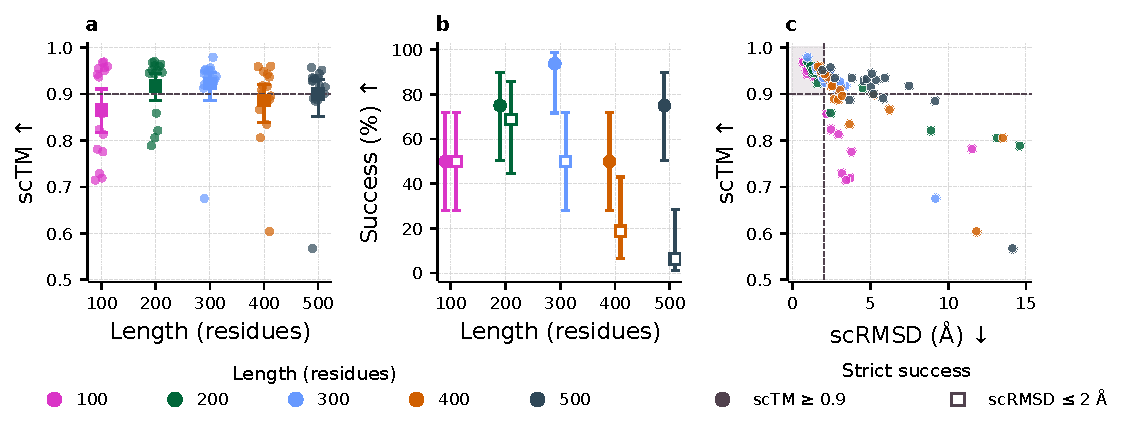
\includegraphics[width=\linewidth]{figures/protein/protein_multimodal_evidence.pdf}
%     \caption{Backbone quality from denoised bits: (a) scTM by length, (b) strict success
%     by length, and (c) fold similarity versus coordinate error. Colours denote length. 80 backbones each receive one ProteinMPNN redesign and ESMFold refold. Intervals are 95\%. Shading marks both strict criteria.}
%     \label{fig:protein:multimodal}
%     \label{fig:protein:strict}
% \end{minipage}\par\addvspace{6pt} 

\begin{figure}[!t]
    \centering
    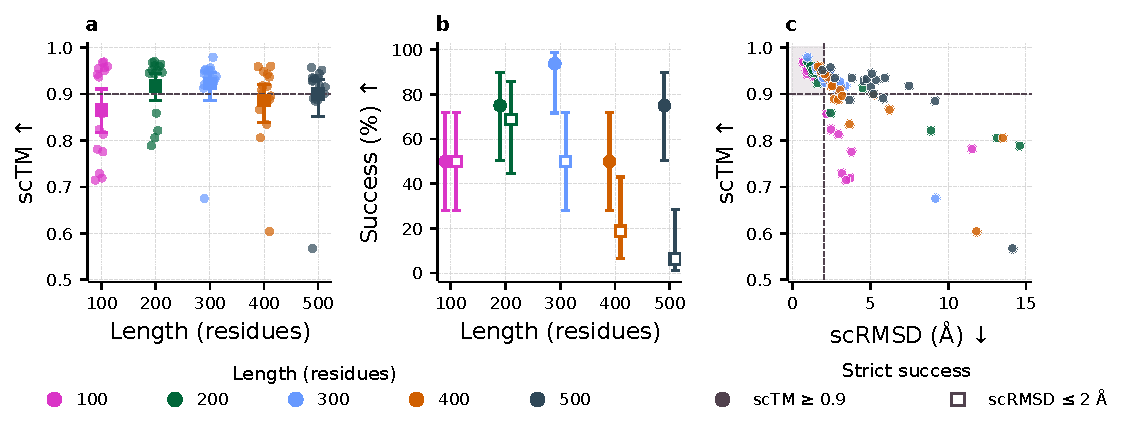
\includegraphics[width=.8\linewidth]{figures/protein/protein_multimodal_evidence.pdf}
    \caption{Backbone quality from denoised bits: (a) scTM by length, (b) strict success
    by length, and (c) fold similarity versus coordinate error. Colours denote length. 100 backbones (20 per length) each receive one ProteinMPNN redesign and ESMFold refold. Intervals are 95\%. Shading marks both strict criteria.}
    \label{fig:protein:multimodal}
    \label{fig:protein:strict}
\end{figure}

% We ask whether one shared bitstream formulation can learn representations of protein sequences and structures. Unlike text, image, and audio multimodality, whose correspondence is primarily semantic, a protein sequence and it's three-dimensional structure are physically coupled descriptions of the same molecualr system. 

% In a given environment,. the amino-acid sequences shapes the protein's free energy landscape and accesible conformation ensemble \cite{protein:anfinsen} while a target backbone restricts the sequences likely to adopt that fold \citep{protein:proteinMPNN}. 

\textbf{Setup.} Clamping either channel gives inverse or forward folding while leaving both free enables joint generation, without task-specific fine-tuning or multiple sequence alignments as input (Appendix~\ref{app:protein:metrics}). Our evaluations were based on entropic DDIM with $50$ grid points, conditional CFG $5$ and no unconditional guidance. Under these settings, mean recovery is $44.10\%$ on 128 CATH 4.3 validation targets and forward TM is $.554$ on $183$ CAMEO targets \citep{protein:cath,protein:cameo,protein:tmscore}. These results test bidirectional learning through one shared bitstream objective. For $100$ generated backbones ($20$ per length, 100--500), one ProteinMPNN redesign and ESMFold refold give mean scTM $.899$ \citep{protein:proteinmpnn,protein:esmfold}. Figure~\ref{fig:protein:multimodal} shows fold similarity across lengths while Figure~\ref{fig:protein:bestgallery} shows the best backbones per length-bucket. We assess backbone recovery after redesign and refolding using scTM  $\geq.9$ ($D_{\mathrm{TM}}$) for overall fold agreement and scRMSD $\leq2$\,\AA{} ($D_{\mathrm{RMSD}}$) for close coordinate agreement. Full metrics and sampling analysis are in Appendices~\ref{app:protein:metrics} and~\ref{app:protein:pareto}. 

Directly refolding CoBit's own sequences for the same 80 pairs gives mean scTM $.911$, with $D_{\rm TM}=69\%$ and $D_{\rm RMSD}=41\%$ (Table~\ref{tab:protein:direct}; Appendix~\ref{app:protein:direct}). This supports sequence--structure consistency at the fold level, despite lower coordinate-level success.


% \textbf{Learning the joint representation.} Clamping one modality gives forward or inverse folding. Leaving both free gives joint generation. \bruno{add the figure for the overview} show the two conditional directions and the generated-backbone evaluation. Information aboout training, evaluation, and the tokenizer can be found in Appendix~\ref{app:protein:protocol}. 

% \par\addvspace{6pt}\noindent
%     \begin{minipage}{\linewidth}
%     \makeatletter\def\@captype{figure}\makeatother
%     \centering
%     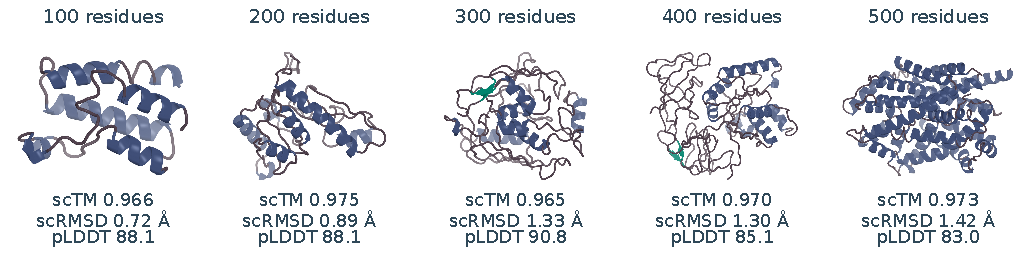
\includegraphics[width=.99\linewidth]{figures/protein/protein_pymol_best_grid.pdf}
%     \caption{Selected CoBit backbones, rendered with PyMOL \citep{protein:pymol}.
%     Highest scTM at each displayed length among samples with scRMSD $\leq2$\,\AA{};
%     scores use ProteinMPNN/ESMFold. pLDDT is predicted confidence.}
%     \label{fig:protein:bestgallery}
% \end{minipage}\par\addvspace{6pt}
\par\addvspace{6pt}\noindent
    \begin{minipage}{\linewidth}
    \makeatletter\def\@captype{figure}\makeatother
    \centering
    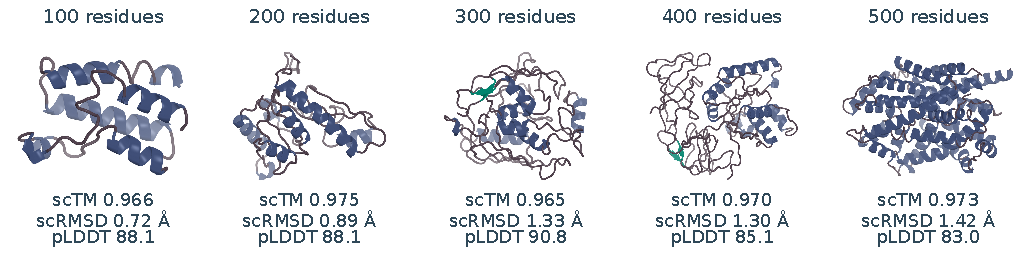
\includegraphics[width=.99\linewidth]{figures/protein/protein_pymol_best_grid.pdf}
    \caption{Selected CoBit backbones, rendered with PyMOL \citep{protein:pymol}.
%     Highest scTM at each displayed length among samples with scRMSD $\leq2$\,\AA{};
    Highest scTM among 20 samples at each displayed length with scRMSD $\leq2$\,\AA{};
    % scores use ProteinMPNN/ESMFold. pLDDT is predicted confidence.
    scores use ProteinMPNN/ESMFold. pLDDT is refold confidence.}
    \label{fig:protein:bestgallery}
\end{minipage}\par\addvspace{6pt}



% Sequence constrains the energy landscape and conformational ensemble \bruno{ cite affinsen....}, while structure constrains funcional vability. Hence, protein co-design goes byeyond cross-modal aligment, but joint generation over discrete sequence and continuous 3D geometry can be achieved with respect to geometric, chemical, thermodynamic and functional constraints intrinsic to these modalities \bruno{Cite Jumper et al.  }. 

% Figures~\ref{fig:protein:strict} and~\ref{fig:protein:lengthdist} show length-dependent quality: high fold similarity does not always imply low coordinate error. Figure~\ref{fig:protein:secondary} shows coarse secondary-structure proportions close

% Protein co-design there requires more than cross-modal semantic alignment because the structure and sequence must be mutually compatible. Cobit addesses this problem by jointly denoising discrete amino0acid and structural codes, with the structural codes being subsequently decoded into continuous backbone coordinates. Structural comparability can be assessed computionally through sequence refolding \citep{protein:jumper, protein:esmfold} whereas thermodynamic stability and biological function require additional computational or even experimental validation \cite{protein:rfdiffusion}, which is beyond the scope of this work. 

\textbf{Bitstream capability versus protein optimisation.} We compare CoBit's bitstream formulation against protein-specific models. Table~\ref{tab:protein:baselines} places CoBit alongside the models evaluated by \citet{protein:simpledesign}, following their published one-redesign procedure with 100 samples. MultiFlow \citep{campbell2024multiflow} leads on the strict criteria with a 21.8M-parameter model that uses explicit geometric learning and designability distillation. On the other hand, CoBit tests the common bit objective with an existing codec and paired-data recipe. Its sequence replay supplies unpaired examples unlike MultiFlow's designability distillation and without direct geometric supervision. Appendix~\ref{app:protein:comparison} explains the training differences and MultiFlow's distillation ablation in detail.


\par\addvspace{6pt}\noindent
\begin{minipage}{\linewidth}
\makeatletter\def\@captype{table}\makeatother
\centering
\begin{minipage}[t]{.55\linewidth}
\vspace{0pt}
\caption{Backbone designability (\%) with one ProteinMPNN redesign and ESMFold.
% Training data and evaluation settings differ across studies. Published baselines: \citet{protein:simpledesign}; G: general bitstream framework; P: protein-specific generator.}
Training data and evaluation settings differ across studies. Published PMPNN1 baselines: \citet{protein:simpledesign}; G: general bitstream framework; P: protein-specific generator.}
\label{tab:protein:baselines}
\label{tab:protein:literaturemain}
\centering
\fontsize{8}{9.5}\selectfont
\setlength{\tabcolsep}{2pt}
\begin{tabular}{@{}rlcrrr@{}}
\toprule
ID & Model & Scope & $n$ & $D_{\rm RMSD}$ & $D_{\rm TM}$ \\
\midrule
\multicolumn{6}{@{}l}{\emph{Our evaluation: joint bitstream generator}} \\
% 1 & CoBit & G & 80 & 38.8 & 68.8 \\
1 & CoBit & G & 100 & 36.0 & 75.0 \\
\midrule
\multicolumn{6}{@{}l}{\emph{Published evaluation: Lu et al. (2026)}} \\
\addlinespace
\multicolumn{6}{@{}l}{Joint generators: discrete structural codes} \\
2 & DPLM-2 (650M) & P & 100 & 31.0 & 48.0 \\
3 & ESM3 Open (sequence first) & P & 100 & 17.0 & 19.0 \\
4 & ESM3 Open (structure first) & P & 100 & 3.0 & 4.0 \\
\addlinespace
\multicolumn{6}{@{}l}{Joint generators: explicit / partially latent geometry} \\
5 & MultiFlow & P & 100 & 86.0 & 90.0 \\
6 & La-Proteina (no-triangle) & P & 100 & 84.0 & 86.0 \\
7 & La-Proteina (triangle) & P & 100 & 84.0 & 88.0 \\
8 & SimpleDesign & P & 100 & 44.0 & 63.0 \\
9 & ProtPardelle & P & 100 & 42.0 & 41.0 \\
10 & ProtPardelle-1c & P & 100 & 52.0 & 53.0 \\
11 & ProteinGenerator & P & 100 & 42.0 & 46.0 \\
\addlinespace
\multicolumn{6}{@{}l}{Structure generators} \\
12 & Proteina & P & 100 & 46.0 & 50.0 \\
13 & RFdiffusion & P & 100 & 49.0 & 54.0 \\
14 & FrameFlow & P & 100 & 46.0 & 49.0 \\
\bottomrule
\end{tabular}
\end{minipage}\hfill
\begin{minipage}[t]{.43\linewidth}
\vspace{0pt}
\makeatletter\def\@captype{figure}\makeatother
\caption{Visual representation of the rates from Table~\ref{tab:protein:baselines}. CoBit captures how proteins fold overall, but is less accurate on fine structural detail.}
\label{fig:protein:modelmap}
\centering
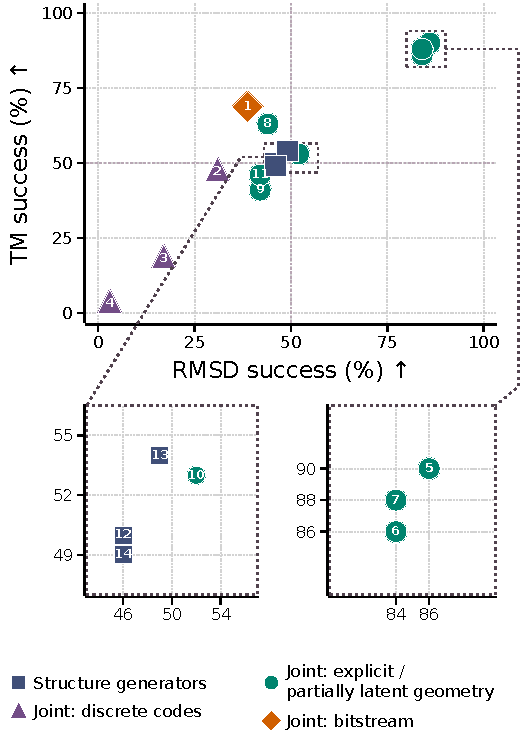
\includegraphics[width=\linewidth]{figures/protein/protein_model_designability_map.pdf}
\end{minipage}
\par\smallskip
\end{minipage}\par\addvspace{6pt}

A dedicated protein study can test that coupling and stronger supervision while testing scalability for biological tasks such as binder--linker design with laboratory (wet lab) validation. CoBit's stronger fold-level ($D_{\mathrm{TM}}$) than coordinate-level ($D_{\mathrm{RMSD}}$) success indicates that denoising structural bits captures useful protein organization information and that geometric precision can be further improved in a dedicated protein-training work, but this is highly dependent, in our case, to protein length and training set availability as shown in Figure~\ref{fig:protein:strict}. The present metrics indicate modeling quality, but establishing biological function requires additional setups and experiments. 

% Under the same training regime, we reach 44.10\% mean amino-avid recovery on CATH 4.3 validation and $.554$ mean forward TM-score \bruno{cite tm-score} on CAMEO 2022 \bruno{cite}, and $0.899$ mean backbone scTM (Table~\ref{tab:protein:headline}). 

% \bruno{Simplify image / reduce space}
% \begin{figure}[t]
%     \centering
%     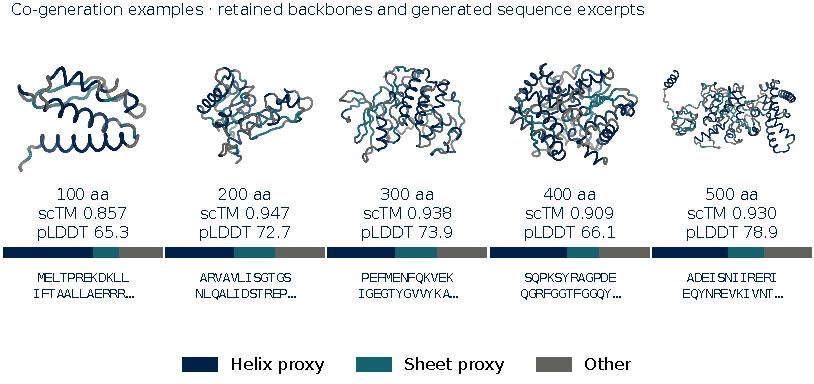
\includegraphics[width=\linewidth]{figures/protein/protein_pymol_gallery.pdf}
%     \caption{Placeholder}
%     \label{fig:protein-pymol-gallery}
% \end{figure}

% % \begin{table}[h!]
% % \centering
% %     \caption{}
% % \label{tab:protein:headline}
% % \small
% % \setlength{\tabcolsep}{4pt}
% % \begin{tabular}{llrl}
% % \toprule
% % Task & Evaluation & $n$ & Results $\uparrow$ \\
% % \midrule
% %     Inverse folding & CATH validation & 128 & AAR 44.10\%; scTM .739 \\
% %     Forward folding & CAMEO 2022 & 183 & TM .554; lDDT .541 \\
% %     Generated backbones & Lengths 100--500 & 80 & scTM .899; $D_{\rm TM}$ 68.75\% \\
% % \bottomrule
% % \end{tabular}
% % \end{table}

% % \begin{table}[h!]
% % \centering
% % \caption{One CoBit model for protein sequence and structure generation.
% % All-candidate means describe typical quality; best-of-four scores describe
% % selection with the native reference.}
% % \label{tab:protein:headline}
% % \small
% % \setlength{\tabcolsep}{3pt}
% % \begin{tabular*}{\linewidth}{@{\extracolsep{\fill}}lrrrrrr@{}}
% % \toprule
% % \multicolumn{7}{@{}l}{\textbf{Inverse folding} --- CATH validation: 128 targets, 512 sequences} \\
% % & & \multicolumn{2}{c}{AAR (\%) $\uparrow$} & \multicolumn{3}{c}{First sequence only: 128 refolds} \\
% % \cmidrule(lr){3-4}\cmidrule(l){5-7}
% % Model & Params (M) & Mean (all) & Best of 4 & scTM $\uparrow$ & scRMSD (\AA) $\downarrow$ & pLDDT $\uparrow$ \\
% % \midrule
% % CoBit & 396.23 & 44.10 & 45.20 & .739 & 6.104 & 61.80 \\
% % \bottomrule
% % \end{tabular*}
% % \end{table}

% \begin{table}[h!]
% \centering
% \caption{Aggregate CoBit quality across three tasks (all metrics $\uparrow$).
% Pure-entropic spacing, $N=50$ and conditional CFG 5.}
% \label{tab:protein:headline}
% \small
% \setlength{\tabcolsep}{3pt}
% \begin{tabular}{@{}rrrrrr@{}}
% \toprule
% \multicolumn{2}{c}{Inverse folding} & Forward folding & \multicolumn{3}{c}{Generated backbones} \\
% \cmidrule(lr){1-2}\cmidrule(lr){3-3}\cmidrule(l){4-6}
% AAR (\%) & Mean scTM & Mean TM & Mean scTM & $D_{\rm RMSD}$ (\%) & $D_{\rm TM}$ (\%) \\
% \midrule
% 44.10 & .739 & .554 & .899 & 38.75 & 68.75 \\
% \bottomrule
% \end{tabular}
% \par\smallskip
% \begin{minipage}{\linewidth}\footnotesize
% Inverse: 128 CATH targets, four sequences/target for AAR and one refold/target for scTM.
% Forward: all four predictions on each of 183 CAMEO targets. Backbones: 80 samples,
% one ProteinMPNN redesign each. $D_{\rm RMSD}$: scRMSD $\leq2$\,\AA{};
% $D_{\rm TM}$: scTM $\geq.9$. Means weight targets equally.
% \end{minipage}
% \end{table}

% Together, these results show that bitstream diffusion supports protein sequence and structure learning. Following the standard backbone-designability protocol, each generated backbone is redesigned once with ProteinMPNN and the resulting sequence is refolded with ESMFold \citep{protein:proteinmpnn, protein:esmfold}, This evaluation asks whether the generated backbone supports a comptaible sequence. Directly refodlng CoBit's simulataneously generated sequence would instead mesure end-to-end co-design consistency and is left for future evaluation. Cobit's strict TM success rate ($68.8\%$) numerically exceeds the DPLM-2/ESM3 \citep{protein:dplm2, protein:esm3} entries (($48.0\%$ and $19.0\%$ respectively) in the published comparison while using fewer denoiser parameters \bruno{table literature}. Sample counts and training data differ, and MultiFlow leads both strict success criteria. These results motivated dedicate training specific tasks like binder--linker design studies, although biological function tests are beyond the scope of this work.

% The complete evaluation sweep cover 120 settings per conditional tasks and 20 distinc unconditional settings. CFG is inactive for all unconditional generation sweeps. At 50 NFE, entropic CFG 5 reaises inverse scTM from $.708$ to $.739$ relative to CGF 0, while sequence diversity falls from $0.392$ to $0.145$. Karras sampling reaches $0.753$ inverse scTM, whereas entropyu gives better generated-bacbone scTM ($0.899 verus 0.884$). 50 NFE seemed to be enough for this tasks as we didn't see significant improvement using 200 NFE (from $0.899$ to $0.903$). \bruno{Write in the appendix the pareto optimiality picture for this}. Appendix~\ref{#} further distill step budges from network calls aand reports paretto frontigers. \bruno{add these appendices}. Appendix~\ref{} shows why protein length and strict RMSD success also matter.  


% \begin{table}[h!]
% \centering
% \caption{Backbone designability with one ProteinMPNN redesign.
% Cross-study context from \citet{protein:simpledesign}.}
% \label{tab:protein:literaturemain}
% \small
% \setlength{\tabcolsep}{3pt}
% \begin{tabular}{@{}lrrrr@{}}
% \toprule
% & & & \multicolumn{2}{c}{Designability (\%) $\uparrow$} \\
% \cmidrule(lr){4-5}
% Model & Params (M) & $n$ & $D_{\rm RMSD}$ & $D_{\rm TM}$ \\
% \midrule
% MultiFlow & 21.8 & 100 & \textbf{86.0} & \textbf{90.0} \\
% La-Proteina (no-triangle) & 158 & 100 & 84.0 & 86.0 \\
% \hdashline
% CoBit (R, ours) & 396 & 80 & 38.8 & 68.8 \\
% \hdashline
% SimpleDesign & NR & 100 & 44.0 & 63.0 \\
% Proteina & $\sim$215 & 100 & 46.0 & 50.0 \\
% DPLM-2 & 650 & 100 & 31.0 & 48.0 \\
% ESM3 Open (sequence first) & 1400 & 100 & 17.0 & 19.0 \\
% \bottomrule
% \end{tabular}
% \par\smallskip
% \begin{minipage}{\linewidth}\footnotesize
% Models are ordered by $D_{\rm TM}$. Bold: column maximum.
% Parameters exclude codecs/judges; NR: not verified.
% Data, counts and judges differ; see Appendix~\ref{app:protein:comparison}.
% \end{minipage}
% \end{table}
% \bruno{re-run with n=100...? Luo et al doesn't say about protein lengths or which sequences. Can be done... but without much gain? All these models are protein-specific. Ours isn't. Explore core differences but mainly on training/validation splits, datasets. Still, we're better than DPLM-2 and ESM-3} 

% \bruno{
%  evaluate Cobit's generated pairs. Currentrly: CObit generates sequence -> ProteinMPNN design a replacement sequence, folds replacement with ESMFOld. Good score means "backbone supports compataible sequence"... but did Cobit supply a comptible sequence itself? How does freely generated pairs perform? Next; keep each original cobit seq-structure pair, fold its sequence with ESMFold, and compare prediction with its decoded structures (scTM + scRMSD). We can update table 1 with that.

% }





% \begin{figure}[h!]
% \centering
% 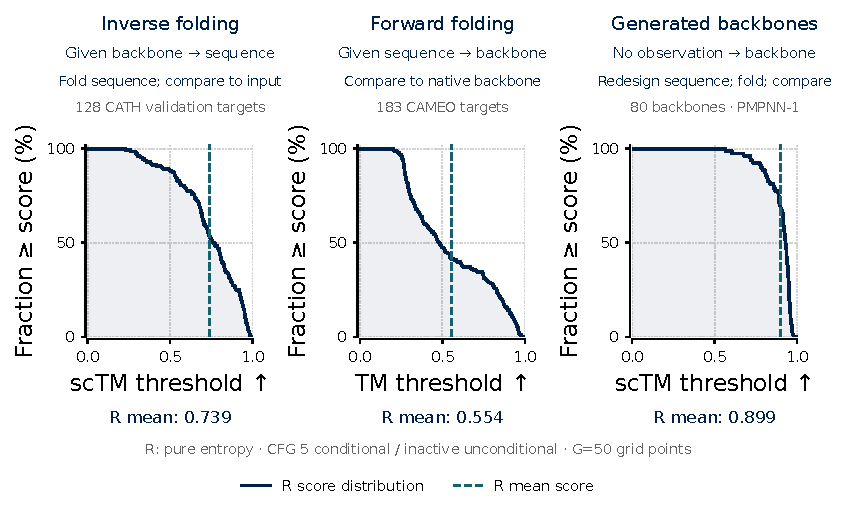
\includegraphics[width=\linewidth]{figures/protein/protein_sampler_overview.pdf}
% \caption{One checkpoint and one recipe R; no sweep maxima are shown.
% Each curve gives the fraction of targets/backbones scoring at least the horizontal
% threshold; dashed lines mark means. Left: one CoBit-sequence refold per CATH target.
% Middle: mean TM of four predictions per CAMEO target. Right: one ProteinMPNN redesign
% per generated backbone, not CoBit's own sequence. Higher curves mean more high-scoring
% examples within a task; the tasks use different references.}
% \label{fig:protein:overview}
% \end{figure}

% \begin{figure}[h!]
% \centering
% 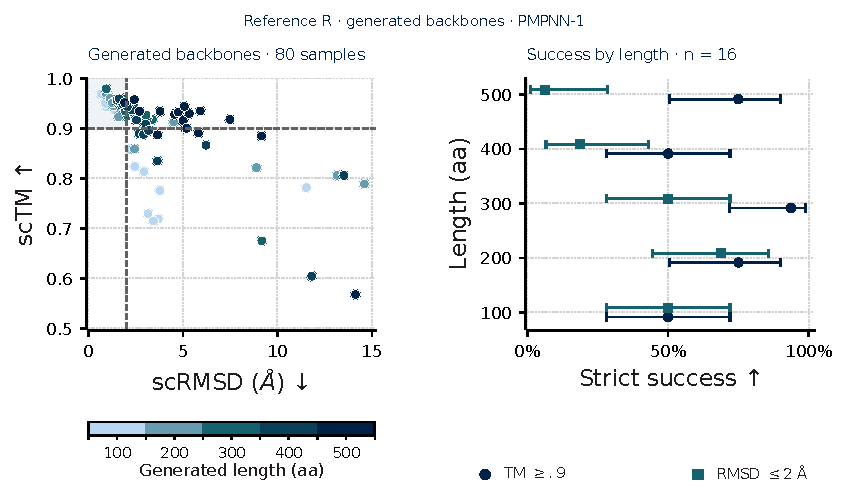
\includegraphics[width=\linewidth]{figures/protein/protein_structure_diagnostics.pdf}
% \caption{Fold similarity and coordinate accuracy are different tests.
% All 80 unconditional backbones use R and one ProteinMPNN redesign followed by ESMFold;
% these are not inverse/forward folding or CoBit-pair scores.
% Left: one dot per backbone, coloured by length; dashed lines mark scRMSD $\leq2$\,\AA{}
% and scTM $\geq.9$, and the shaded region passes both.
% Right: success fractions at each length (16 samples), with 95\% Wilson intervals.
% High TM success at long lengths does not imply low RMSD.}
% \label{fig:protein:strict}
% \end{figure}

% \begin{figure}[h!]
% \centering
% 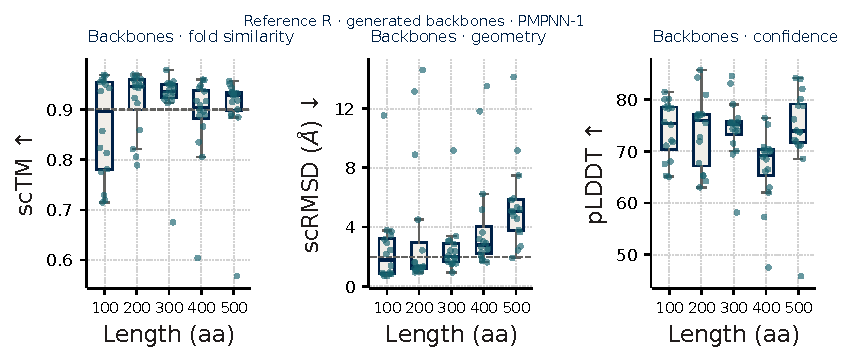
\includegraphics[width=\linewidth]{figures/protein/protein_length_distributions.pdf}
% \caption{Backbone quality across lengths 100--500 at R, using the same 80 samples
% and ProteinMPNN-1/ESMFold judge as Figure~\ref{fig:protein:strict}.
% Every dot is one backbone (16 per length); jitter only separates points.
% Boxes show medians and interquartile ranges; whiskers reach observations within
% 1.5 interquartile ranges. All outliers remain visible.
% Dashed lines mark strict TM/RMSD gates; pLDDT is predicted confidence, not experimental validation.}
% \label{fig:protein:lengthdist}
% \end{figure}

% \begin{figure}[h!]
% \centering
% 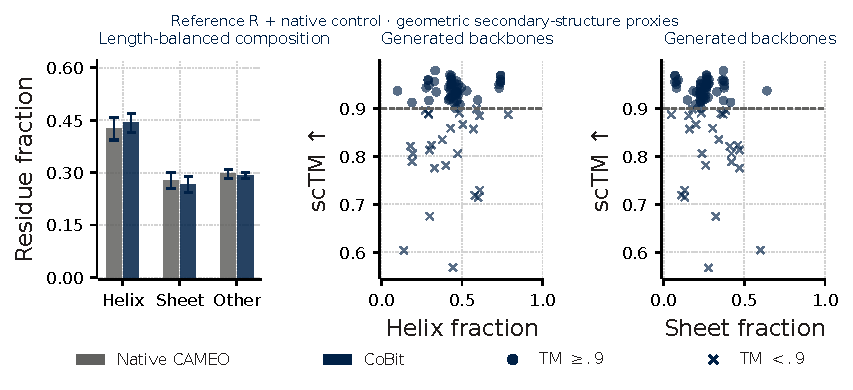
\includegraphics[width=\linewidth]{figures/protein/protein_secondary_structure.pdf}
% \caption{Coarse secondary-structure composition and backbone designability at R.
% Left: mean fractions for 80 generated backbones and 92 native CAMEO controls,
% equally weighted across five length groups; error bars are stratified 95\% bootstrap intervals.
% Middle/right: individual helix-like/sheet-like fractions versus ProteinMPNN-1 scTM;
% circles meet scTM $\geq.9$, crosses do not.
% These C$\alpha$ geometry proxies are not DSSP assignments, and the control is not the full PDB.
% Similar composition alone does not establish naturalness or function;
% details are in Appendix~\ref{app:protein:secondary}.}
% \label{fig:protein:secondary}
% \end{figure}
\endgroup
